\documentclass[12pt]{article}
\usepackage[a4paper]{geometry}
\usepackage[utf8]{inputenc}
\usepackage[T1]{fontenc}
\usepackage[english]{babel}
\usepackage{mathtools}
\usepackage{amsfonts}
\usepackage{amsmath}
\usepackage{hyperref}
\usepackage{subcaption}
\usepackage[dvipsnames]{xcolor}
\hypersetup{
    colorlinks=true,
    linkcolor=RoyalPurple,   
    urlcolor=RoyalPurple
}

\title{Oscilloscope vector graphics on a \mbox{Telequipment D54} using an \mbox{Arduino MKR Vidor 4000}}
\author{Teodora Osiac \and Ioan Dragomir}
\date{January 2021}

\begin{document}

\makeatletter
\renewcommand{\and}{\quad}
\begin{titlepage}
	\vspace*{\fill}
	\centering

	\makeatletter
	\centering{\LARGE\bfseries \@title \par} \vspace{1.5cm}

	
\includegraphics[height=1.5in]{images/tucn-logo.jpg}\par

	\vspace{1.5cm}
	{\Large\@author \par}\vspace{0.45cm}

	{\large supervised by\par
	Prof. Dr. Radu Fechete}

	\vspace*{\fill}
	{\large \@date\par}
\end{titlepage}
\makeatother

\begin{abstract}
\noindent Displaying line art on an oscilloscope in XY mode is a common entry level electronics project, which is much beloved by hobbyists worldwide, both for the ease of obtaining minimally functional graphics, as well as the plentiful challenging enhancements it often requires. We aim to display arbitrary animations at a smooth frame rate (50Hz), with a resolution finer than the trace width (cca. 0.5mm), and covering as much of the 10x6cm screen of the Telequipment D54 as possible. Breaking down the system we identify six successive steps from concept to displayed graphics: Graphics design, Path optimisation, Compressed encoding, Transmission, Decompression, Signal generation and display, each of which can be individually optimised once some general parameters are established, such as the expected resolution. <TODO: overview results>

\end{abstract}

\setcounter{tocdepth}{2}
\tableofcontents

\section{Introduction}

Mama tata

\section{Background}

TODO: Cover various kinds of DACs, especially the limitations of PWM with smoothing, gray code DACs which prevent glitches, sigma-delta DACs, etc

TODO: Cover other similar projects and Jerobeam Fenderson's music as inspiration

\section{Signal generation, display characteristics}

To confirm the feasibility of the project, we start with a rudimentary software stack that enables programming an Arduino with a fixed, two-channel waveform corresponding to the X and Y coordinates of a point walking along a given path. At the hardware level, we require two DACs of sufficient resolution, which motivates our choice of the Arduino MKR Vidor 4000, since it has a builtin 10-bit DAC, meaning we only have to implement a single DAC externally.

One of the requirements for a pleasant and smooth appearance is that we have control over the position of the beam in increments smaller than half the width of the beam itself. (Fig. \ref{fig:low-resolution}) By some crude measurements, our device's beam is approximately 0.5 -- 0.6mm in diameter. To span 6cm vertically in increments less than 0.25mm, we require 240 distinct voltage levels, and thus at least 8 bits resolution for the vertical channel. Similarly, the horizontal channel requires at least \( \log_2{10\text{cm}/0.25\text{mm}} \approx 8.6 \) bits. Therefore we chose to use the built-in 10-bit DAC for the horizontal channel and to build an external 8-bit DAC for the vertical channel.

DAC design choice is a significant factor in both circuit complexity, cost, and the quality of the resulting graphics. We chose an R-2R design for its relative simplicity, in spite of the expected DAC glitches (Fig. \ref{fig:vertical-dac-glitches}) that appear when passing between points at a large Hamming distance but small Euclidean distance. (i.e., at coordinates at 1/2, 1/4, 3/4, etc. vertically within the screen)

\begin{figure}
\centering
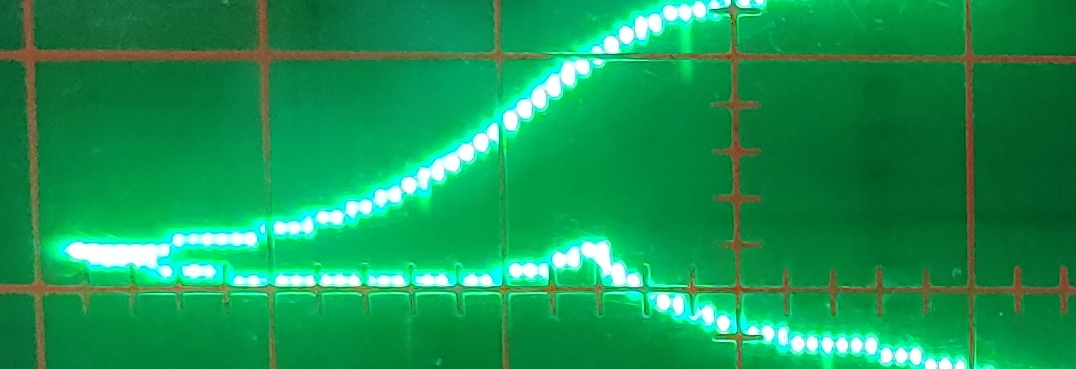
\includegraphics[width=0.8\textwidth]{images/low-resolution.png}\quad
\caption{Low resolution leads to noticeable discrete points}
\label{fig:low-resolution}
\end{figure}

\begin{figure}
\centering
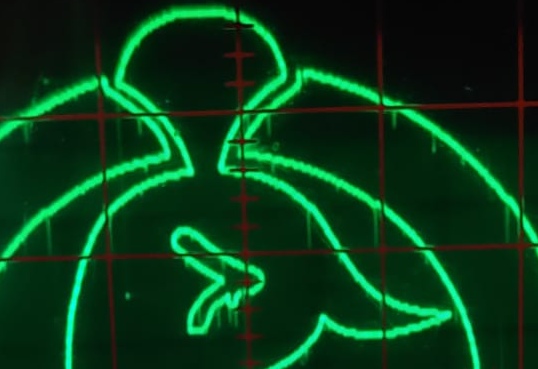
\includegraphics[width=0.4\textwidth]{images/vertical-dac-glitches1.png}\quad
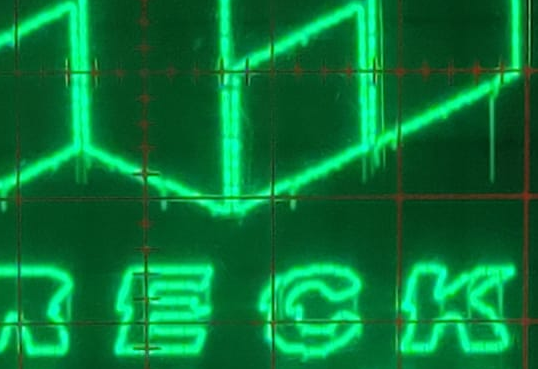
\includegraphics[width=0.4\textwidth]{images/vertical-dac-glitches2.png}
\caption{Vertical DAC glitches look like spikes at certain Y values}
\label{fig:vertical-dac-glitches}
\end{figure}


\section{Transmission benchmarking}

How fast can we transmit stuff over USB to the Arduino?

\section{Compressed encoding and decoding}

Given transfer rate limits, test some compression schemes both in: how many points can they send per frame (one 50th of a second)? how fast can the arduino decompress the data once sent?

We suppose the controlling computer has enough computational power for it not to matter. Latency is also not an issue as long as the output refresh rate is consistent.

\section{Path optimisation}

2OPT with a custom path distance function and like 100 random starting positions to get a relatively ok path in the end

\section{Graphics design}

??????????????? How do we actually design/make animations ?????????


\end{document}
